\section{Pilottest til valg af gestikker}
\label{PilottestValgAfGestikker}
%
Der udføres en pilottest, for på den måde at finde og eliminere fejl i testdesignet. Formålet med pilottesten er at undersøge, hvorvidt de forskellige aspekter i testen fungerer og om der opstår komplikationer, eksempelvis ved at optage testpersonerne. Baseret på pilottesten vil det være muligt at foretage ændringer såfremt der opstår komplikationer eller andre problemer.\blankline
%  
Til pilottesten blev der testet på fire studerende, der ellers ikke lever op til kriterierne for at være testperson, jævnfør \fullref{TestpersonerValgAfGestikker}. Årsagen til at disse testpersoner blev testet er både, at de var tilgængelige og at formålet med pilottesten er at teste forskellige aspekter såsom videoerne, spørgeskemaet, instruktionerne og testlederen samt observatørens position. Resultaterne fra pilottesten fremgår af \autoref{app:ResultaterPilottestValgAfGestikker}. Baseret på resultaterne fra pilottesten, bekræftes antagelsen om, at studerende med en forhåndsviden om design, brugertest og lignende samt studerende, hvis hovedfokus er på elektronik og software, ikke er i stand til at give upåvirket respons. To af testpersonerne vælger gestikker med udgangspunkt i deres teknologiske baggrund og ikke nødvendigvis ud fra hvad de faktisk foretrækker.\blankline
% 
Under pilottesten blev der optaget med et Canon Powershot s110, som ikke formåede at holde strøm tilstrækkeligt lang tid. Optagelserne fra pilottesten blev derfor enten afbrudt for tidligt eller slet ikke optaget, da kameraet løb tør for strøm. Det vælges derfor at optagelserne fremadrettet vil foregå med et GoPro Hero4 Silver kamera.\blankline
% 
Når testpersonerne opfordres til at gengive deres forbedringer til musik, både ved de individuelle videoer og afslutningsvist, så blev musikken afspillet igennem iTunes på den computer, hvor observatøren tager noter. Herved opstod der et problem, da det ikke var alle musiknumre i iTunes, som startede med det samme, hvilket forårsagede forvirring for testpersonerne, som ikke vidste om de havde gjort noget forkert. Det vælges derfor at opsætte en afspilningsliste med musiknumre, som alle starter med det samme, så der fremover ikke opstår tvivl om, hvorvidt der skiftes musiknummer. 

Da testpersonerne blev opfordret til at gengive forbedringerne rettede de sig mod observatøren, formentligt fordi testpersonerne registrerede, at det var observatøren, som styrede musikken. Observatørens position ændres derfor, så testpersonerne ikke længere har direkte mulighed for at se observatøren tage noter og styre musikken. Observatørens nye position fremgår af \autoref{fig:TestopstillingPostPilot}.
\newpage 
%
\begin{figure}[H]
	\centering
	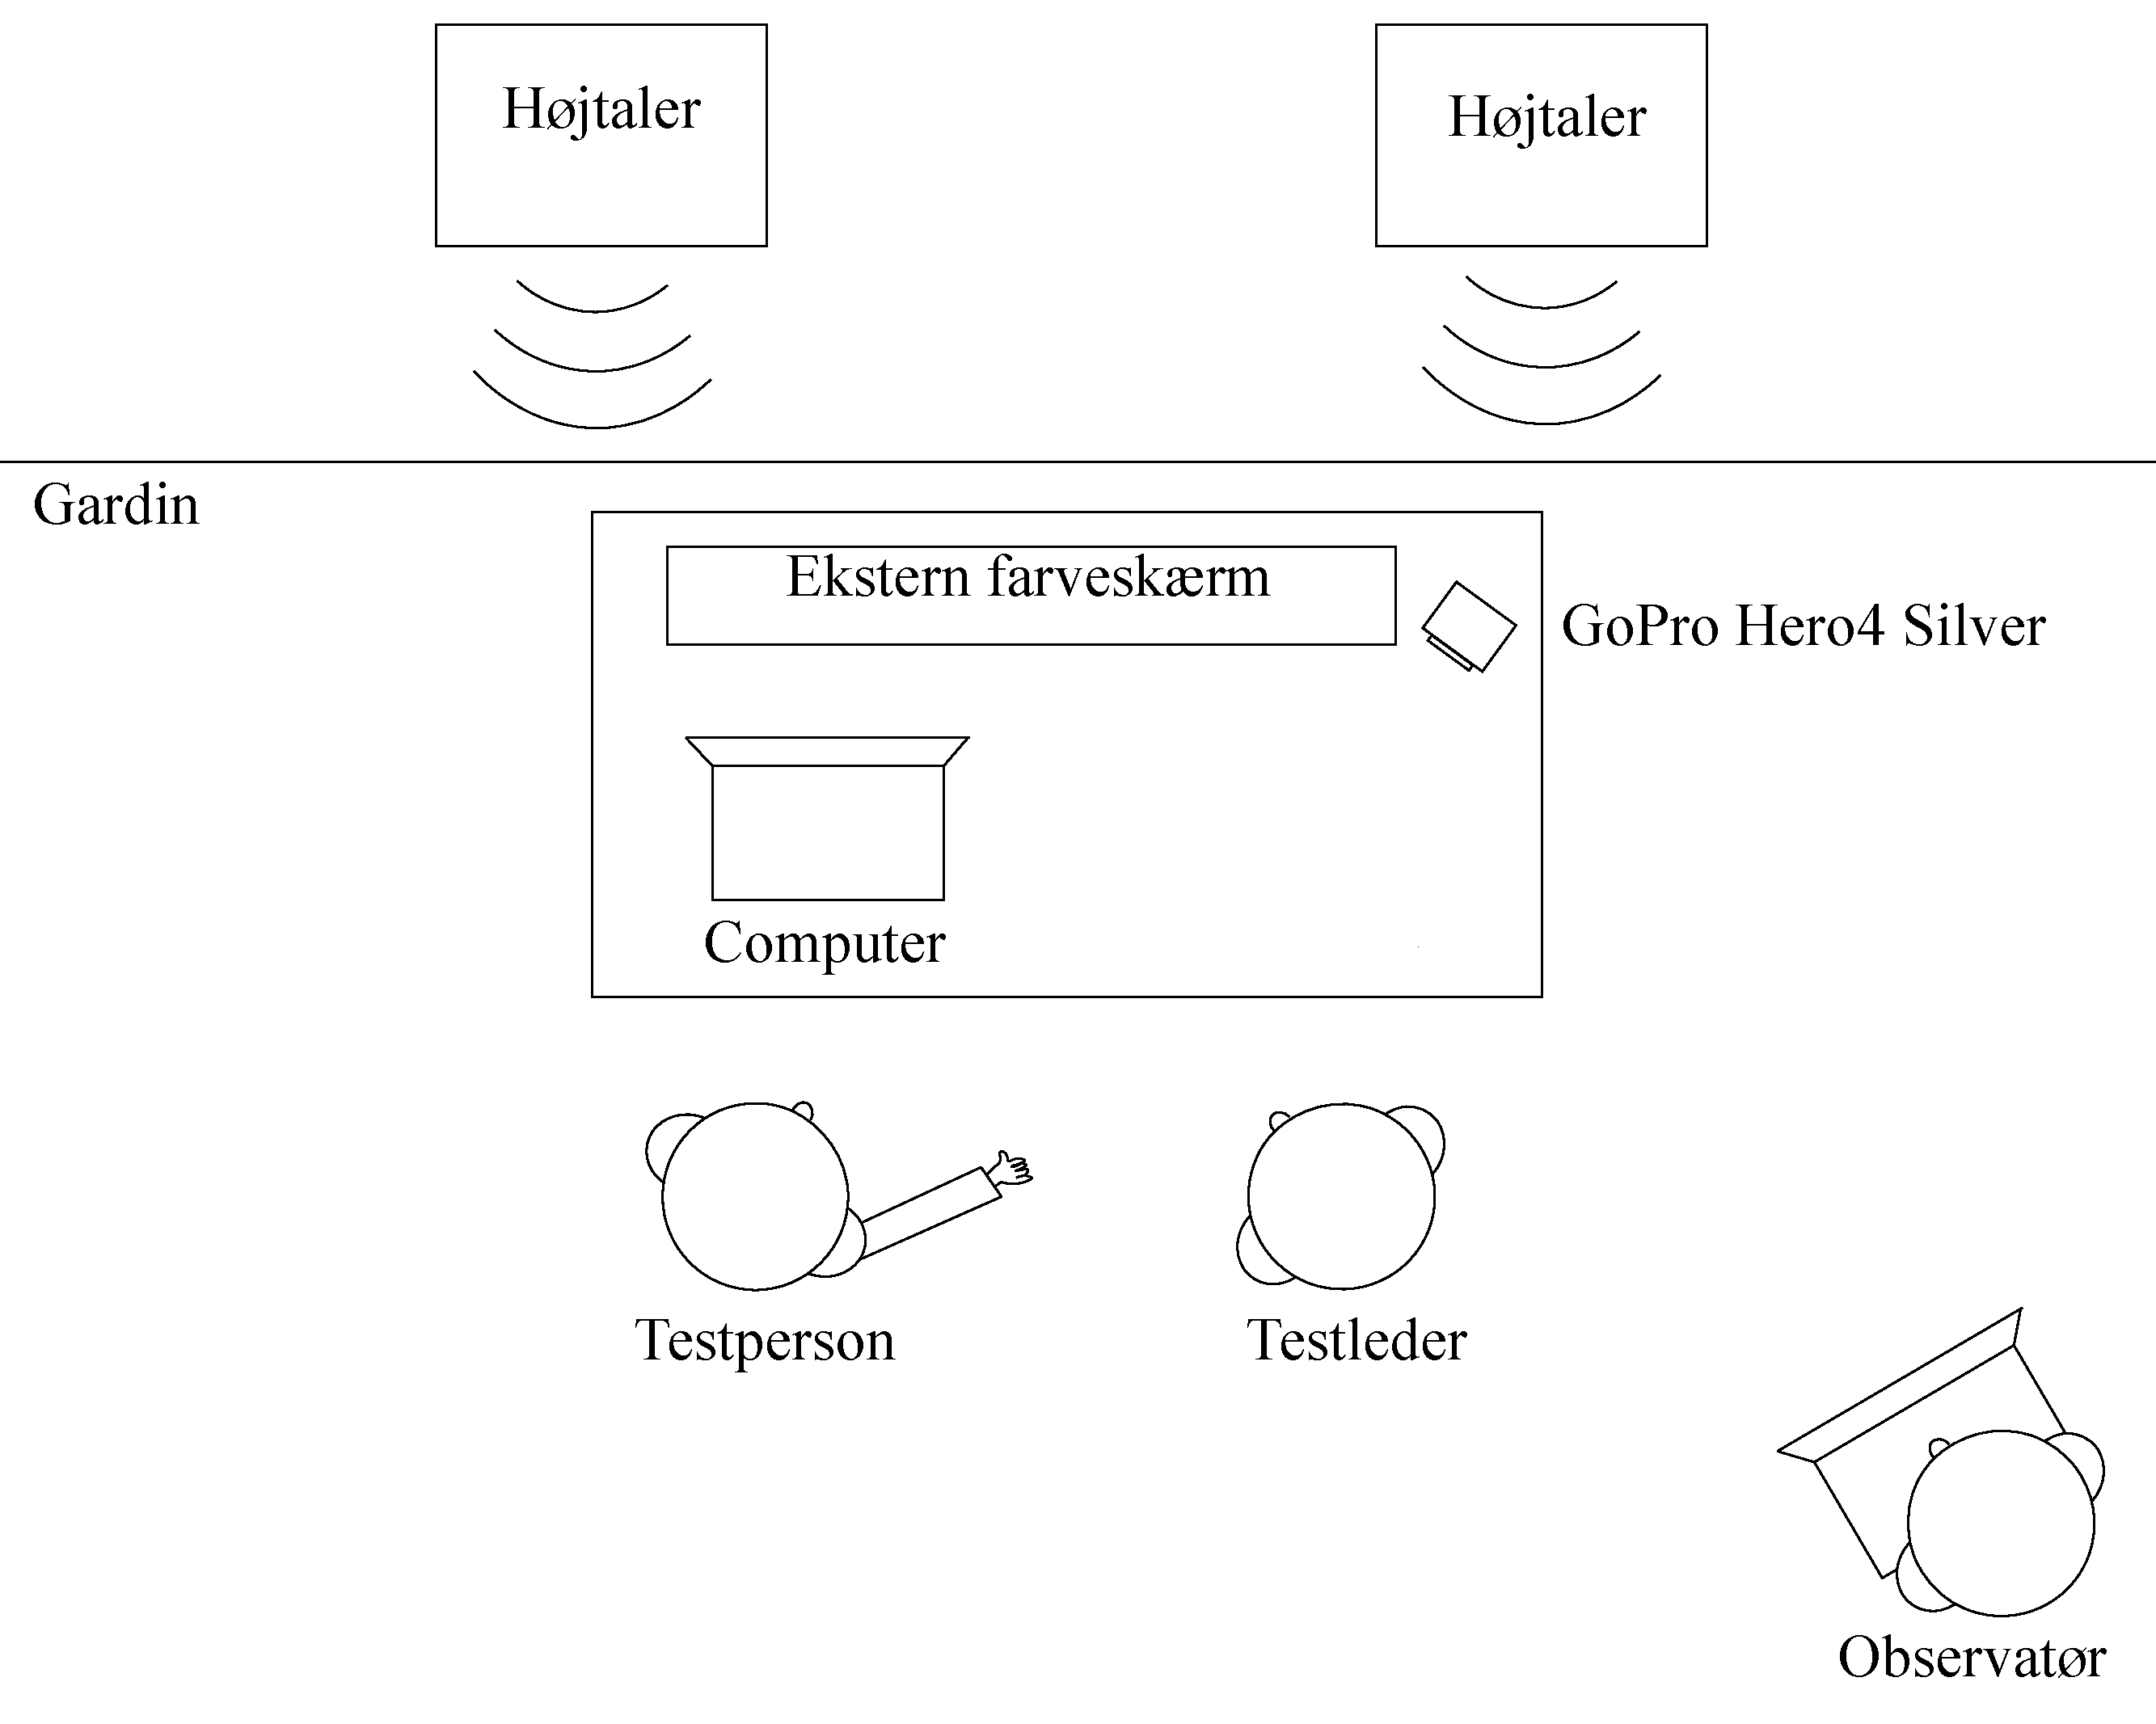
\includegraphics[resolution=300,width=0.8\textwidth]{Test1/TestopstillingPostPilot}
	\caption{Testopstilling hvor placeringen af både observatør og kamera er ændret, samt typen af kamera.}
	\label{fig:TestopstillingPostPilot}
\end{figure}
\noindent
% 
Ydermere blev spørgeskemaet redigeret to gange, så det blev klart for testpersonerne, at det var brugen af gestikker, hvor der ikke røres ved en skærm, der blev spurgt ind til. \blankline
%
Med disse forbedringer vurderes det, at testens forskellige aspekter fungerer.  
 

